%
% Vanadium Avo Logo Design
%

\documentclass{standalone}
\usepackage[dvipsnames]{xcolor}
\usepackage{tikz}

\pgfmathsetmacro{\dPhase}{5}
\pgfmathsetmacro{\waveCount}{10}

\newcommand{\perturbation}[1] {
	\x/3 + 0.02 * \x * cos(6 * \x r + #1 * 15))
}

\def\primaryColor{NavyBlue}
\def\secondaryColor{OrangeRed}

\begin{document}
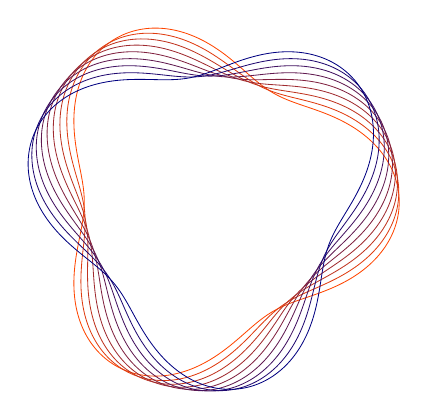
\begin{tikzpicture}[line cap=round, line join=round]
	\pgfmathsetmacro{\circleX}{2.8 * pi + 2}
	\pgfmathsetmacro{\waveCount}{8}
	\foreach \i in {0, ..., \waveCount} {
		\pgfmathsetmacro{\blend}{(\i / \waveCount) * 100}
		\draw[\primaryColor!\blend!\secondaryColor, line width=0.3pt, smooth, samples=200, domain=0:2*pi] plot (
			{cos(\x r + \i * 5) *	(2 + cos(\x r * 3) * 0.4)},
			{sin(\x r + \i * 5) *	(2 + cos(\x r * 3) * 0.4)}
      		);
	}
\end{tikzpicture}
\end{document}
